% Chapter Template

\chapter{Organic Semiconductors} % Main chapter title

\label{Chapter2} % Change X to a consecutive number; for referencing this chapter elsewhere, use \ref{ChapterX}

\lhead{Chapter 2. \emph{Organic Semiconductors}} % Change X to a consecutive number; this is for the header on each page - perhaps a shortened titl

\section{Introduction}

Organic molecular solids have attracted attention for a variety of applications, as structural materials, in medicine and as semiconductors, for classical transistor applications as OFETs (Organic Field Effect Transistors), or in optoelectronics as OLED (Organic Light Emitting Diode) display materials and OPV (Organic Photovoltaics) solar cells.

One of the issues with photovoltaic materials is the Shockley-Queisser limit, which is a theoretical limit for the efficiency of a solar cell. We exploit interesting properties of organic materials to overcome this limit to get highly efficient solar cells, specifically singlet fission and upconversion. Materials such as Y6 have showcased impressive efficiencies near 20\%  [cite].

\section{Excited States}

In organic materials, we are interested in two types of excited states : singlets and triplets. 

Excited singlet states are formed when an electron gets excited such that the overall spin quantum number s = 0 (the multiplicity hence being 2s + 1 = 1)

% Diagram for singlet state in a dimer. 

Excited triplet states are formed when an electron gets excited such that the overall spin quantum number s = 1 (the multiplicity hence being 2s + 1 = 3). 

% Diagram for triplet state in a dimer.

For the example a dimer, the excited state can also form a charge transfer (CT) state.



\section{Singlet Fission}

% Try writing the entirety of Smith-Michl 2010, 2013 and Casanova 2018 here in your own words. This should bulk up the document by a significant amount.


Singlet fission is a photophysical process that may allow us to improve photoconversion efficiencies in solar cells. This is a downconversion photophysical process where an excited singlet state evolves into two spin-triplets, often observed in organic materials \cite{casanova2018theoretical} \cite{smith2010singlet}.

\begin{equation}
    S^{*} \to T_1 + T_1
\end{equation}

\begin{figure}
\centering
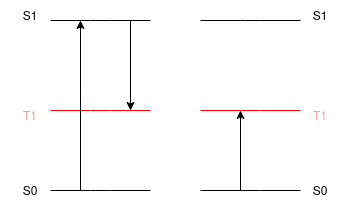
\includegraphics[scale=0.6]{Figures/SF.png}
\caption{Singlet Fission process in a dimer of chromophores}
\end{figure}

As is the case in other internal conversion processes in organic materials it can be very fast, happening at a sub-$ps$ time scale. Despite a large amount of research being devoted to research in singlet fission in organic materials we do not fully understand the mechanisms that underlie this process. 

Singlet fission was first observed by Singh and Stoicheff in 1963 [cite] when they identified intermediate states in anthracene that were able to absorb two photons. Subsequently in the 1960s and 70s, several articles were published around understanding the decay of singlet states into a pair of triplet states and the reverse process, where triplet states annihilate to generate singlets. Kinetic models were developed to try to model singlet fission but were not very successful at reproducing the experimental findings. Since then, more sophisticated electronic structure theories and computational power have allowed for more accurate calculations. In 2006, Hanna and Nozik suggested that singlet fission might help overcome the Shockley-Queisser detailed balance limit \cite{hanna2006solar}, which was the first indication that studying singlet fission might help develop better organic solar cells, the hope being that energy losses from conversion of kinetic energy of excited states of carriers to heat would be mitigated by the generation of a second excited state (with energies at least doubling the band gap). This was a major impetus that stimulated singlet fission research again.


For devices to surpass the Shockley-Queisser limit, they require a SF material capable of absorbing energetic photons and a chromophore to convert solar radiation into an electon-hole pair per photon. To get charge separation in triplet excitons, the use of a material that combines an SF donor and acceptor has shown to be effective. Pentacene-$C_{60}$ heterojunction interfaces have shown promise in ionizing the triplets \cite{rao2010exciton}.



\section{Triplet Annihilation}


\section{Pentacene}

\section{Rubrene}

\section{Y6}

\section{Charge Transport}

\cite{oberhofer2017charge}


\subsection{Band Regime}

\subsection{Hopping Regime}

\subsection{Intermediate Regime}